\documentclass[tikz,border=2pt]{standalone}
\usepackage{amsmath,amssymb}
\usepackage{pgfplots}
\pgfplotsset{compat=1.18}

\begin{document}
% The geometric pmf with p = 0.3 (number of failures before the first success): each extra
% failure multiplies the probability by 1 - p, so the bars decay geometrically from k = 0.
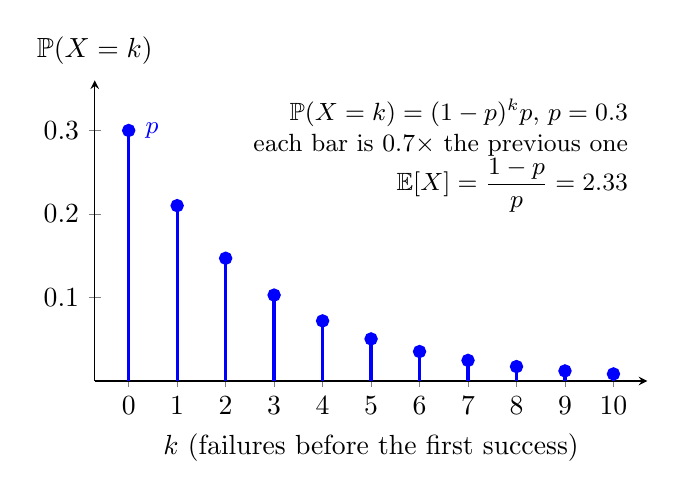
\begin{tikzpicture}
	\begin{axis}[
		axis lines=left, xmin=-0.7, xmax=10.7, ymin=0, ymax=0.36,
		xtick={0,...,10}, ytick={0.1,0.2,0.3},
		xlabel={$k$ (failures before the first success)}, ylabel={$\mathbb{P}(X=k)$}, ylabel style={rotate=-90, anchor=south, at={(axis description cs:0,1.02)}},
		width=8.6cm, height=5.4cm, clip=false
		]
		\addplot[ycomb, blue, very thick, mark=*, mark size=1.8pt] coordinates {(0,0.3000) (1,0.2100) (2,0.1470) (3,0.1029) (4,0.0720) (5,0.0504) (6,0.0353) (7,0.0247) (8,0.0173) (9,0.0121) (10,0.0085)};
		\node[anchor=north east, font=\small, align=right] at (axis cs:10.5,0.35) {$\mathbb{P}(X=k)=(1-p)^kp$, $p=0.3$\\ each bar is $0.7\times$ the previous one\\ $\mathbb{E}[X]=\dfrac{1-p}{p}=2.33$};
		\node[blue, anchor=west, font=\small] at (axis cs:0.15,0.3) {$p$};
	\end{axis}
\end{tikzpicture}
\end{document}
